\documentclass{article}

\usepackage{caption}
\usepackage{subcaption}
\usepackage{graphicx}
\usepackage{tikz}
\usepackage{tikzsymbols}
\usetikzlibrary{calc}
\usepackage{float}
\usepackage{pdflscape}
\usepackage{geometry}
\geometry{a4paper, landscape, margin=1cm}

\def\centerarc[#1](#2)(#3:#4:#5){\draw[#1] ($(#2)+({#5*cos(#3)},{#5*sin(#3)})$) arc (#3:#4:#5);}

\pagestyle{empty}
\begin{document}
	\centering
	\begin{figure}[H]
		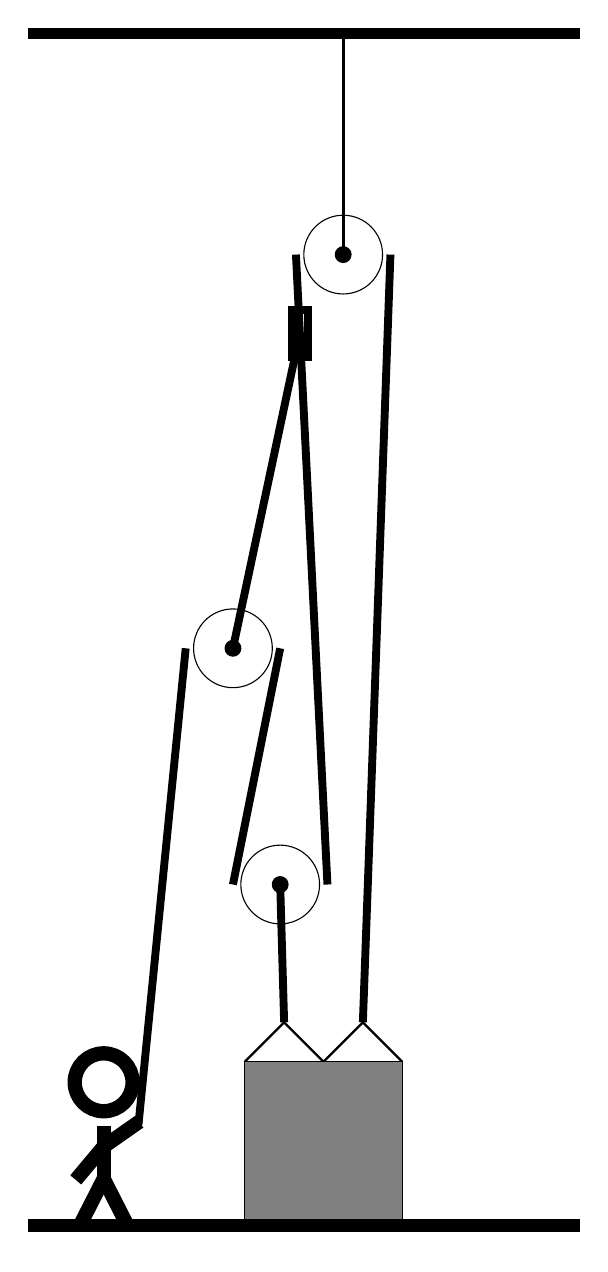
\begin{tikzpicture}
			%%%%% START %%%%%
			\def\a{12}
			\def\radlg{\radrp - 0.1}
			\def\radrp{0.6}
			\def\radsm{0.1}
			\def\xone{0.6}
			\def\yone{\a - 7.75}
			\def\xtwo{1.2}
			\def\ytwo{\a - 10.75}
			\def\xthree{2}
			\def\ythree{\a-2.75}
			\def\xfour{1.45}
			\def\yfour{\a-3.75}
			\def\dx{-1}
			\def\dy{-1.9}
			\def\dw{1.75mm}
			\def\xbox{0.75}
			\def\ybox{-1}
			\def\width{1mm}
			
			\draw[fill=black] (-2,\a) rectangle (5,\a+0.125);
			
			\draw (\xone,\yone) circle (\radlg);
			\draw[fill=black] (\xone,\yone) circle (\radsm);
	
			\draw (\xtwo,\ytwo) circle (\radlg);
			\draw[fill=black] (\xtwo,\ytwo) circle (\radsm);
			
			\draw (\xthree,\ythree) circle (\radlg);
			\draw[fill=black] (\xthree,\ythree) circle (\radsm);
			\draw[very thick] (\xthree,\ythree) -- (\xthree,\a);

			\draw[thick]  (\xbox,\ybox) -- (\xbox+0.5,\ybox+0.5) -- (\xbox+1,\ybox) -- (\xbox+1.5,\ybox+0.5) -- (\xbox+2,\ybox);
			\draw[fill=black!50] (\xbox,\ybox) rectangle (\xbox+2,\ybox-2); 

			\draw[line width=\width] (\dx+0.4,\dy+0.1) -- (\xone-\radrp,\yone);
			\draw[line width=\width] (\xone,\yone) -- (\xfour,\yfour);
			\draw[line width=\width](\xfour-0.1,\yfour-0.3) rectangle (\xfour+0.1,\yfour+0.3); 
			\centerarc[line width=\width](\xone,\yone)(0:180:\radrp);
			\draw[line width=\width] (\xone+\radrp,\yone) -- (\xtwo-\radrp,\ytwo);
			\centerarc[line width=\width](\xtwo,\ytwo)(180:360:\radrp);
			\draw[line width=\width](\xtwo,\ytwo) -- (\xbox+0.5,\ybox+0.5);
			\draw[line width=\width] (\xtwo+\radrp,\ytwo) -- (\xthree-\radrp,\ythree);
			\centerarc[line width=\width](\xthree,\ythree)(0:180:\radrp);
			\draw[line width=\width] (\xthree+\radrp,\ythree) -- (\xbox+1.5,\ybox+0.5);
			
			\node at (-1,-2) {\Strichmaxerl[10][50][35]};
			
			\draw[fill=black] (-2,-3) rectangle (5,-3.15);
			%%%%% END %%%%%
		\end{tikzpicture}
	\end{figure}
	
\end{document}